\section{Membuat Akun Github}
Github merupakan salah satu repository yang populer pada kalangan developer saat ini. Hal ini dikarenakan Github dapat menyimpan project-project open source mereka dimana project tersebut dapat dikembangkan oleh programmer lain baik sebagai team, maupun individual. Disaat kita melakukan perubahan terhadap suatu project, kemudian perubahan tersebut diupload ulang (push) ke repository, maka project yang lama masih tersipan dan tidak akan hilang. Hal ini memudahkan kita untuk melihat dan menganalisa setiap perubahan yang dilakukan sebelumnya. 

Sebelum mempelajari lebih dalam mengenai github, disini akan dijelaskan bagaimana cara membuat akun git pada github :
\begin{enumerate}
\item Pertama, buka browser dan masukkan alamat github dengan url :\textbf{ https://github.com} seperti pada gambar \ref{url}
\begin{figure}[!htbp]
\centerline{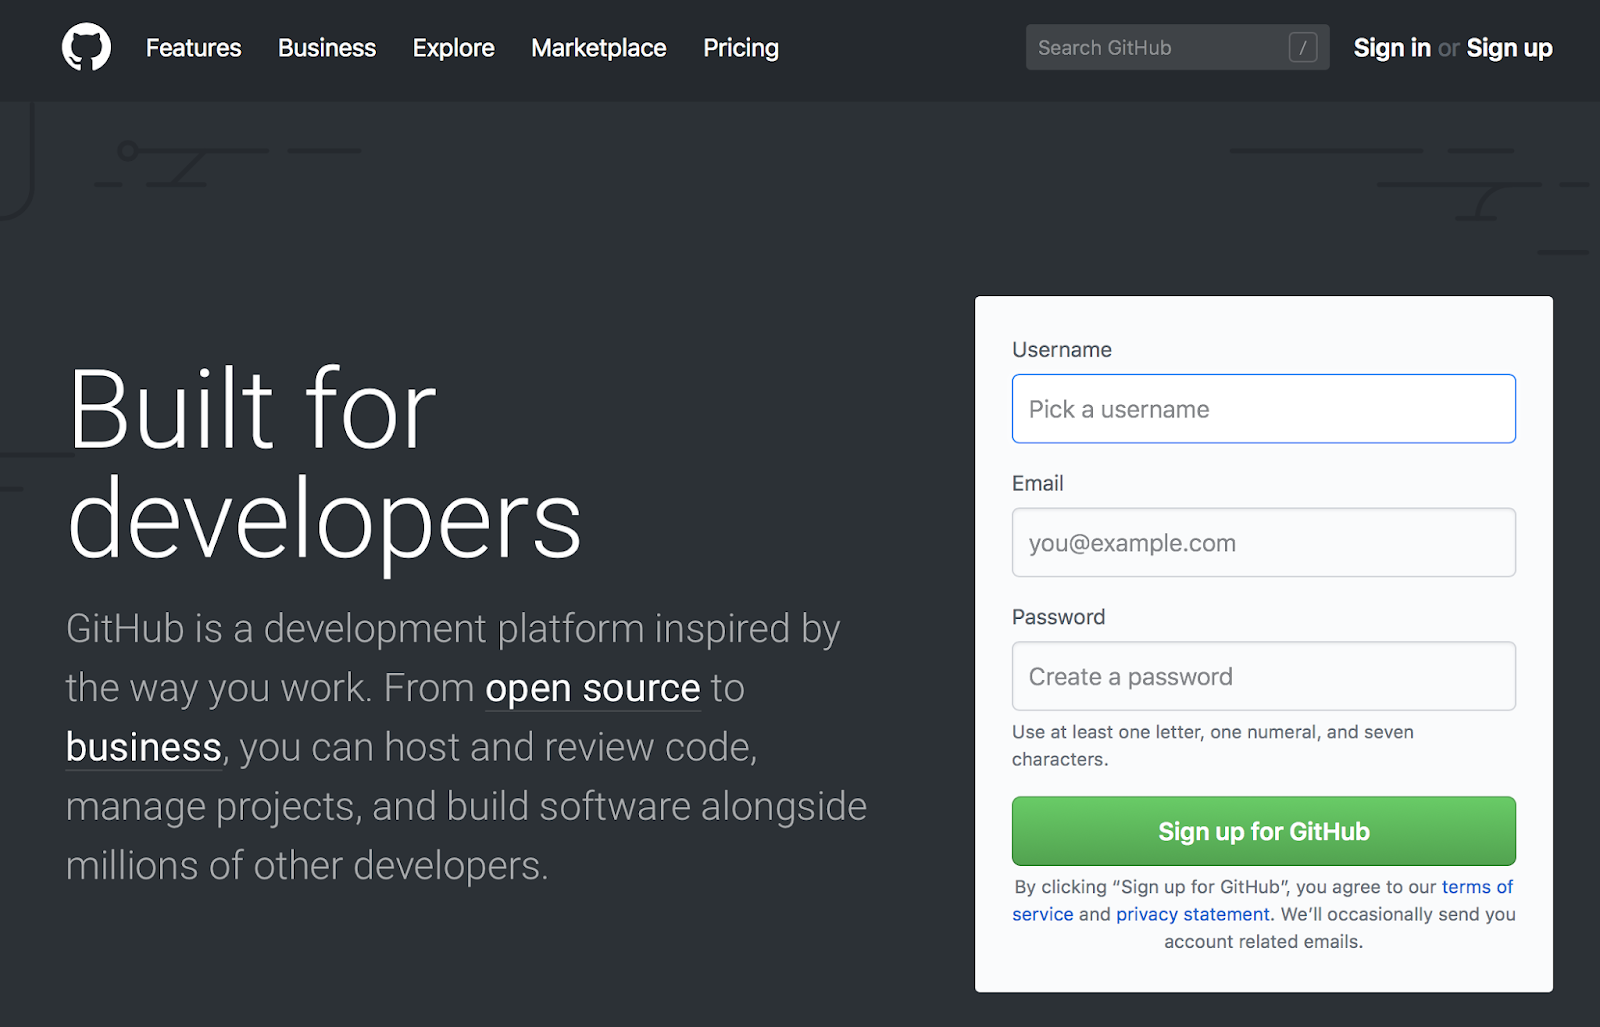
\includegraphics[width=.75\textwidth]{Figures/akunGit/1.PNG}}
\caption{URL Github}
\label{url}
\end{figure}
\item Kemudian masukkan nama user yang akan didaftarkan sebagai akun Github seperti pada contoh \ref{daftar}
\begin{figure}[!htbp]
\centerline{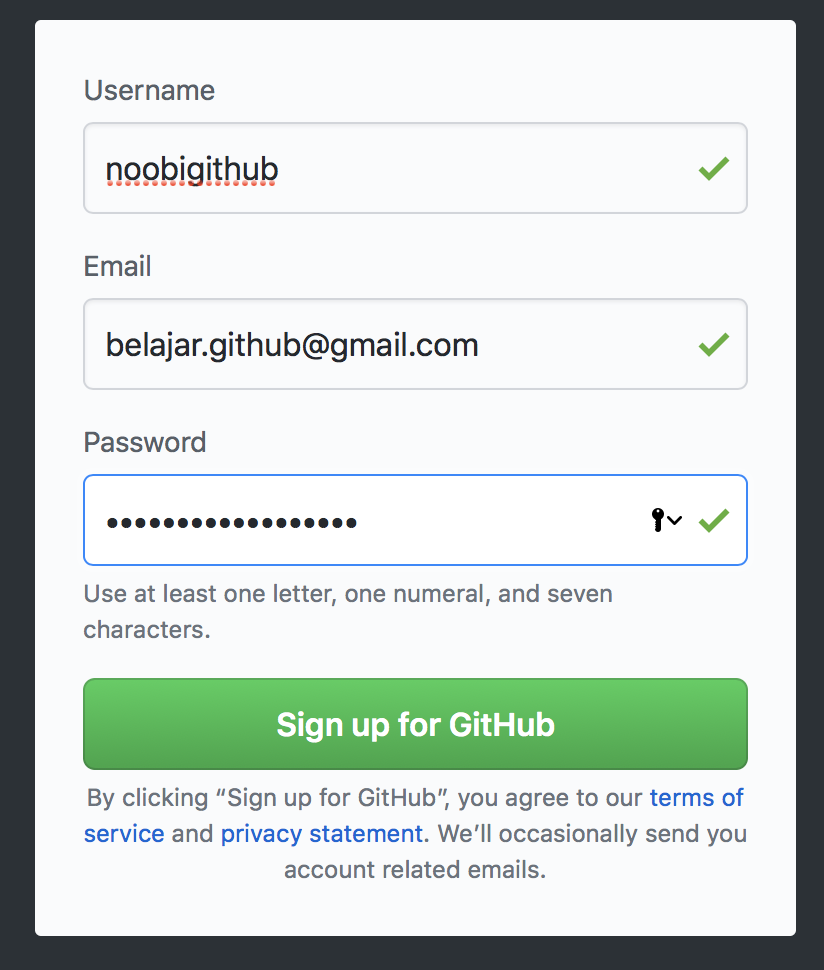
\includegraphics[width=.75\textwidth]{Figures/akunGit/2.PNG}}
\caption{Data yang akan didaftarkan}
\label{daftar}
\end{figure}
\item Setelah memasukkan username dan alamat email, selanjutnya masukkan password yang akan digunakan untuk login github
\item Setelah itu klik tombol sign up for Github dan kita akan diarahkan pada halaman seperti pada gambar \ref{home}
\begin{figure}[!htbp]
\centerline{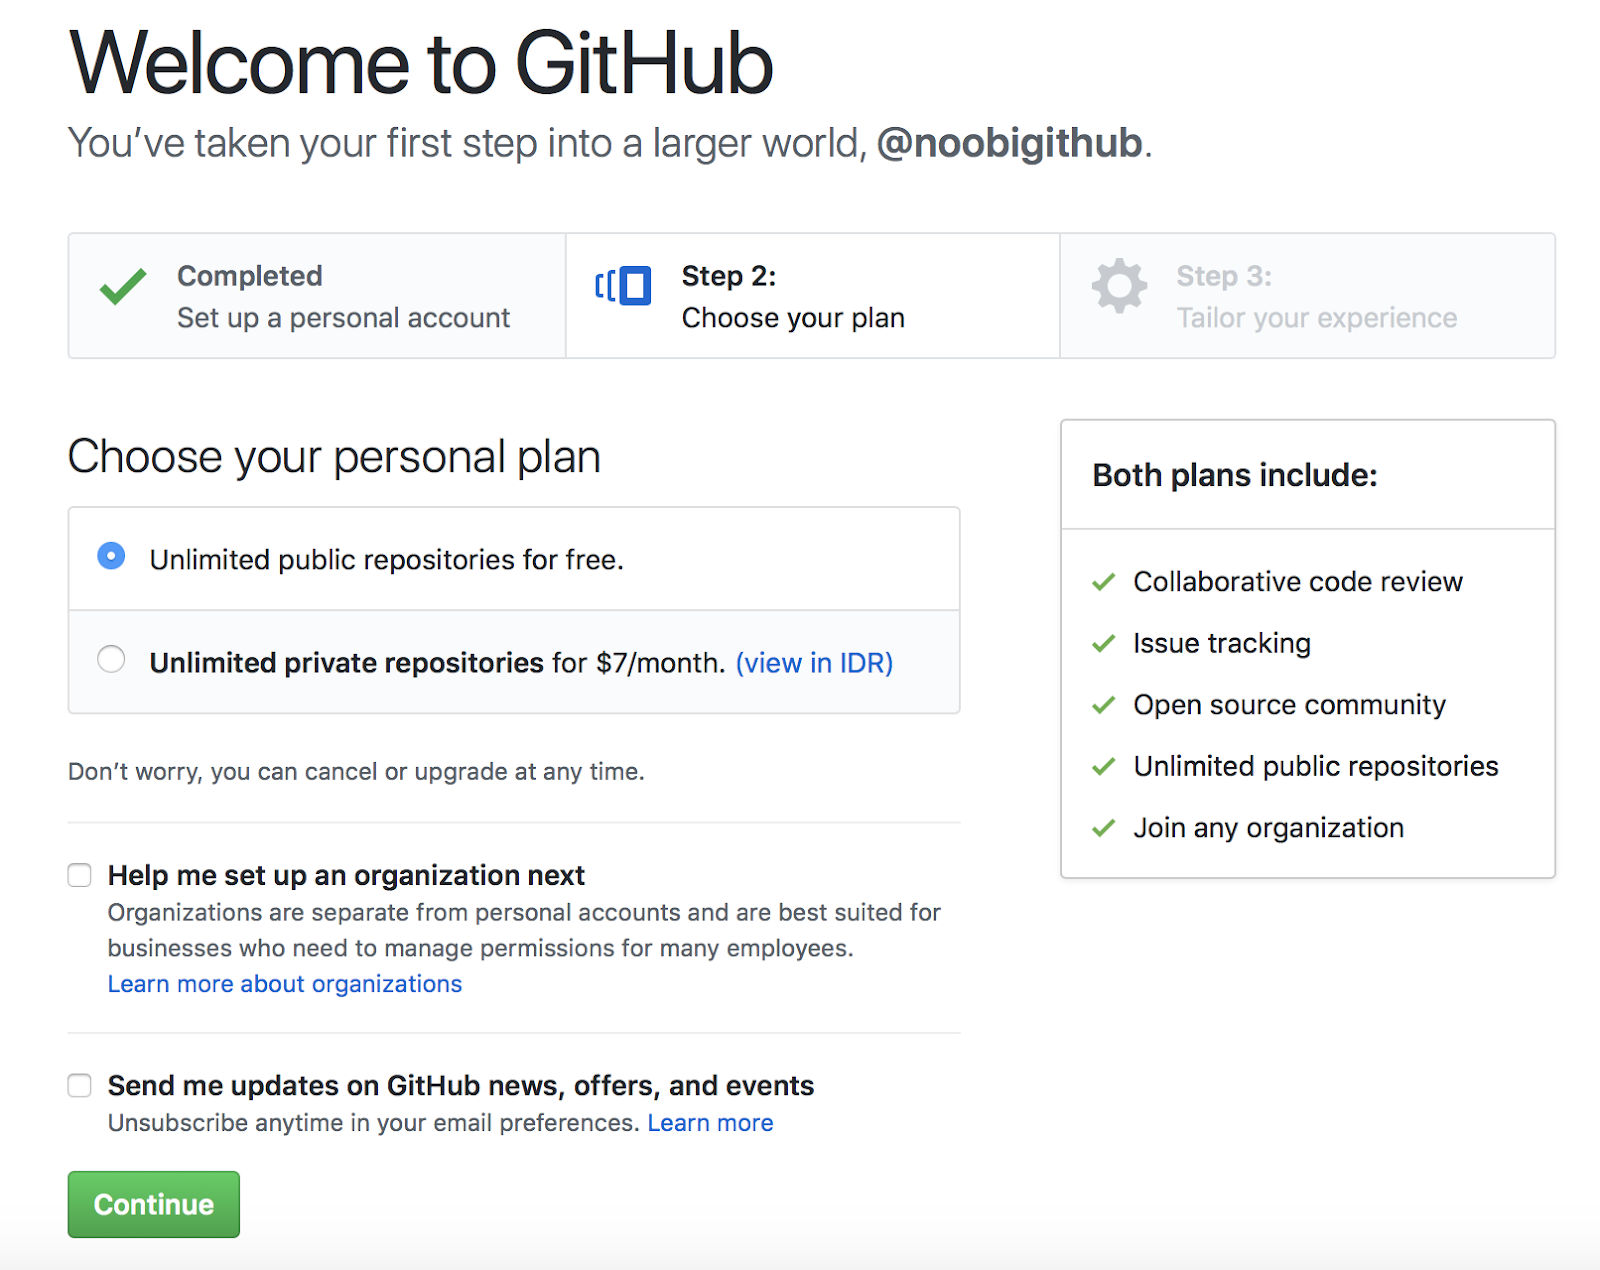
\includegraphics[width=.75\textwidth]{Figures/akunGit/3.PNG}}
\caption{Welcome To Github}
\label{home}
\end{figure}
\item Halaman tersebut akan meminta kita untuk memilih rencana penggunaan repository pada github. Apakah kita akan menggunakan private repository atau public repository (Berbayar atau Gratis)
\item Private Repository memungkinkan repository yang kita gunakan pada github tidak terlihat oleh pengguna lainnya selain pengguna yang didaftarkan sebagai kolabolator
\item Sedangkan pada Public Repository pengguna lainnya dapat melihat repository yang kita miliki. Pada tutorial ini yang akan perlihatkan adalah Public Repository
\item Setelah memilih Public Repository kemudian klik continue untuk melanjutkan pembuatan akun github tersebut. Dan setelah di klik, maka akan diarahkan ke dalam halaman seperti pada gambar \ref{4}
\begin{figure}[!htbp]
\centerline{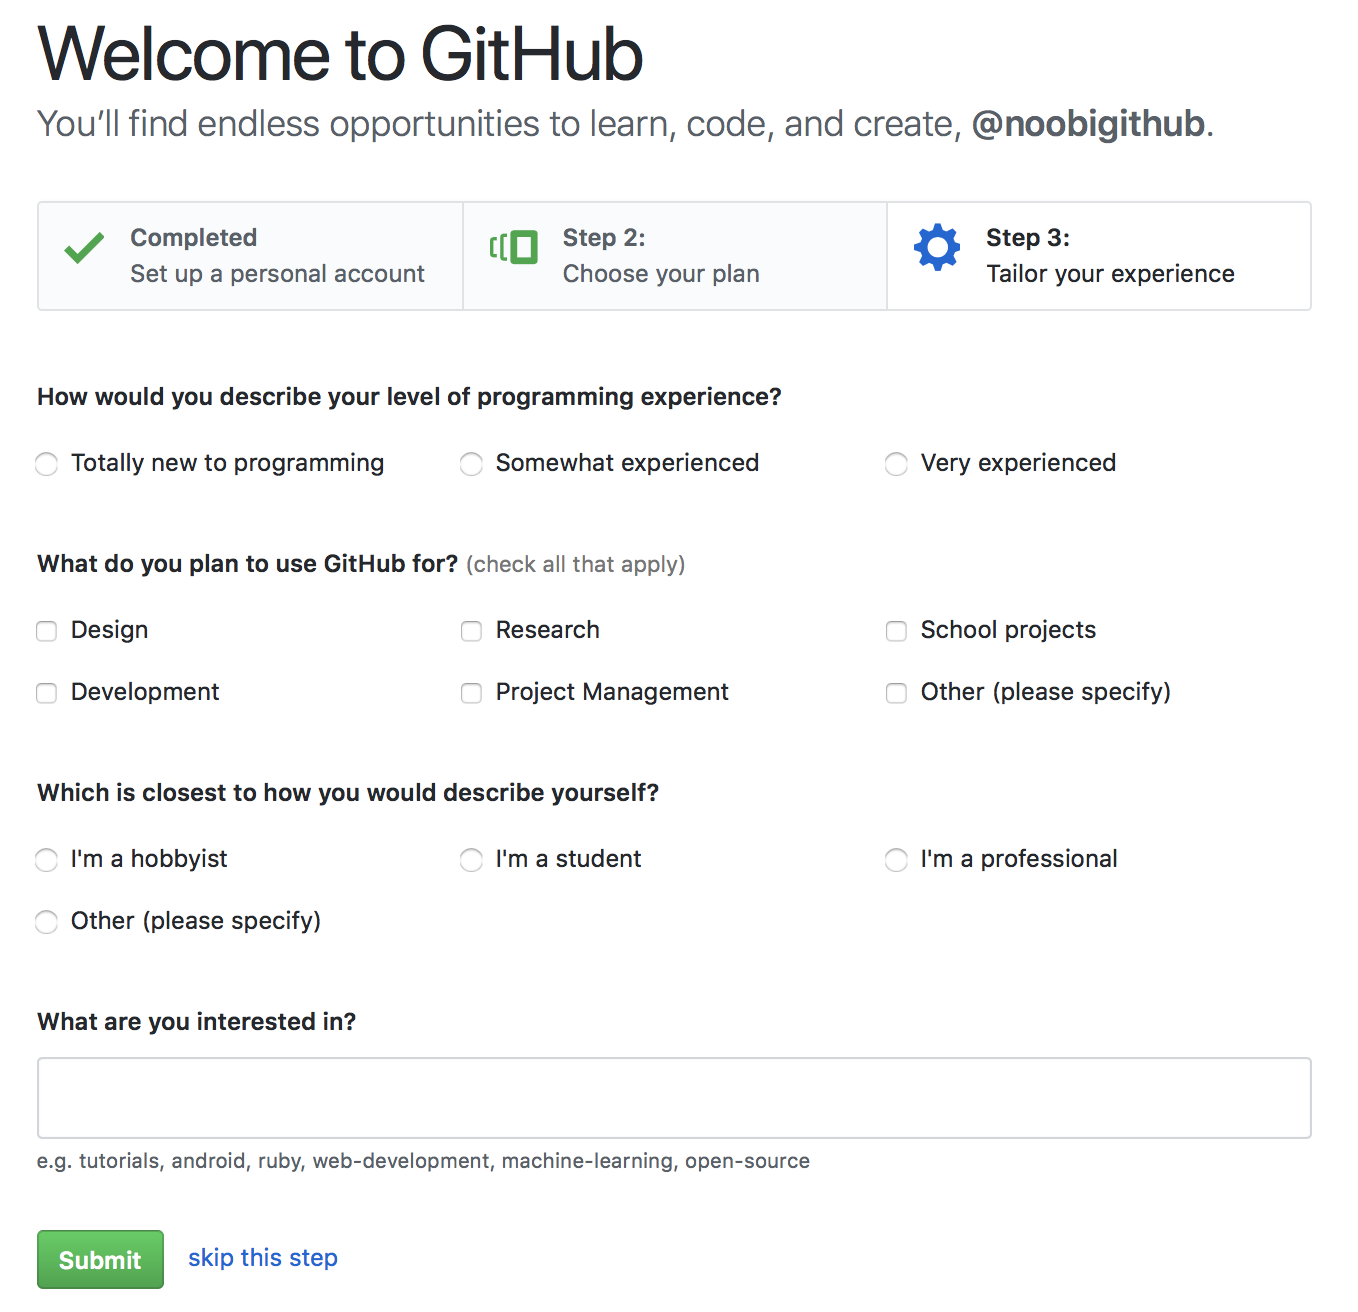
\includegraphics[width=.75\textwidth]{Figures/akunGit/4.PNG}}
\caption{Step pada pembuatan Github}
\label{4}
\end{figure}
\item Pada halaman selanjutnya kita akan diminta untuk memasukkan data profil user yang akan digunakan pada Github
\item Setelah memasukkan data profil kita telah berhasil membuat akun di Github dan akan diarahkan pada halaman seperti pada gambar \ref{5}
\begin{figure}[!htbp]
\centerline{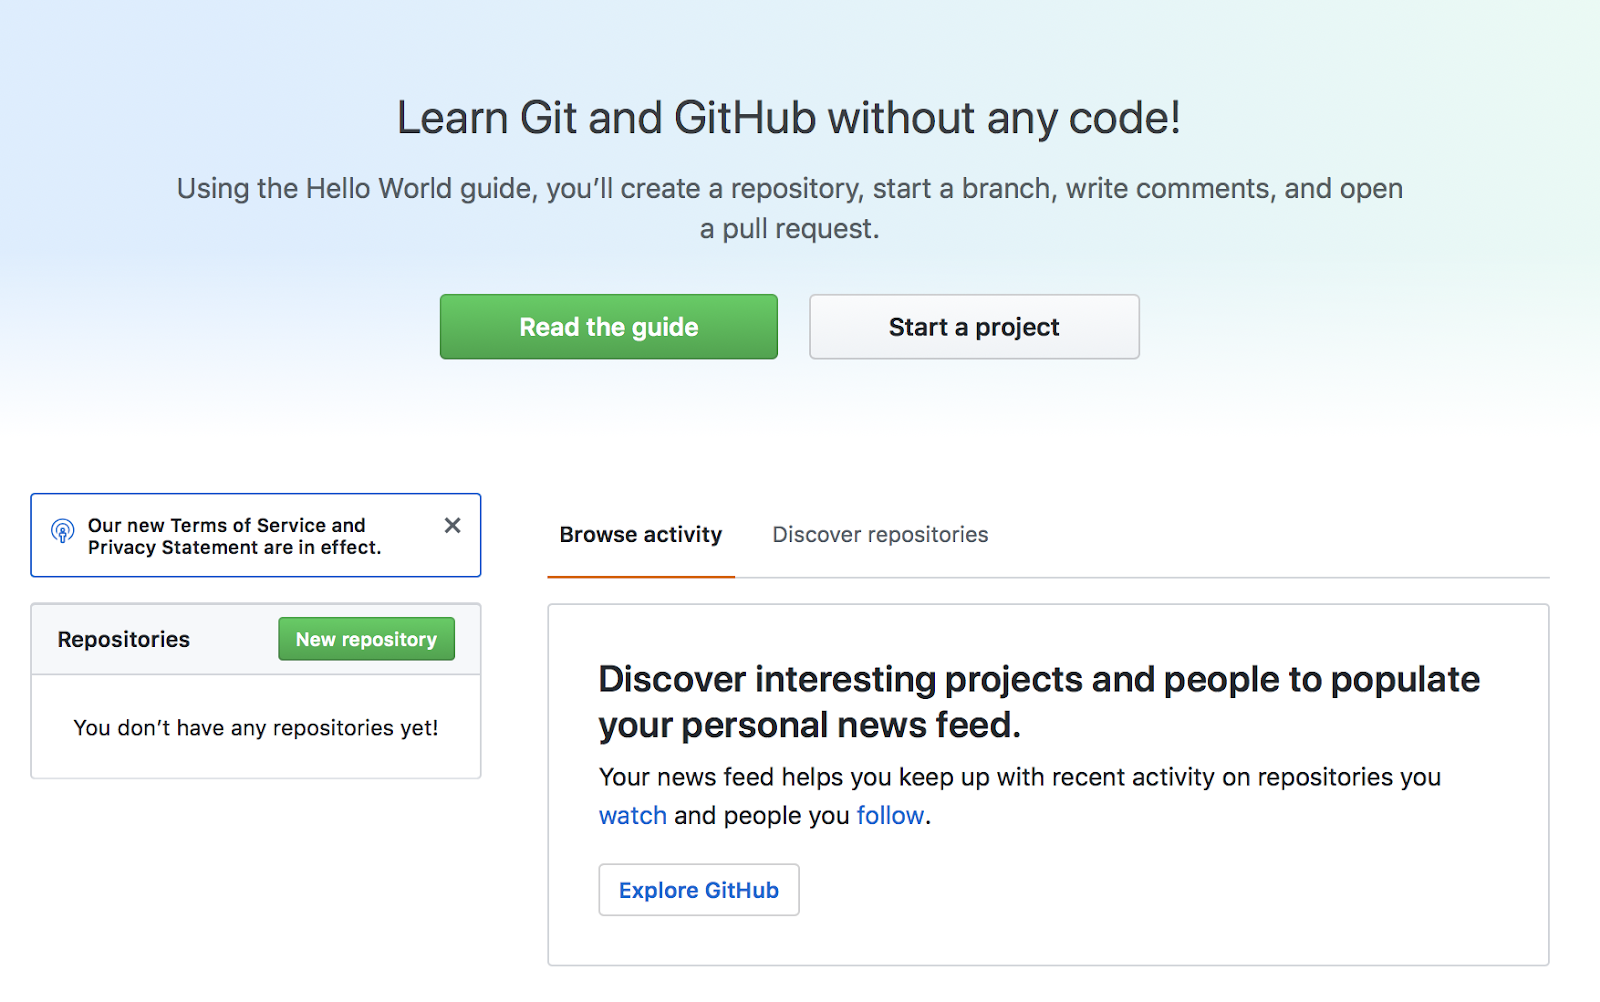
\includegraphics[width=.75\textwidth]{Figures/akunGit/5.PNG}}
\caption{Akun Github Berhasil dibuat}
\label{5}
\end{figure} 
\item Setelah berhasil membuat akun github, kita sudah siap untuk membuat repository baru didalamnya
\item Gambar \ref{6} merupakan menu yang digunakan untuk menampilkan repository yang kita buat atau repository yang mendatarkan kita sebagai kolabolator
\begin{figure}[!htbp]
\centerline{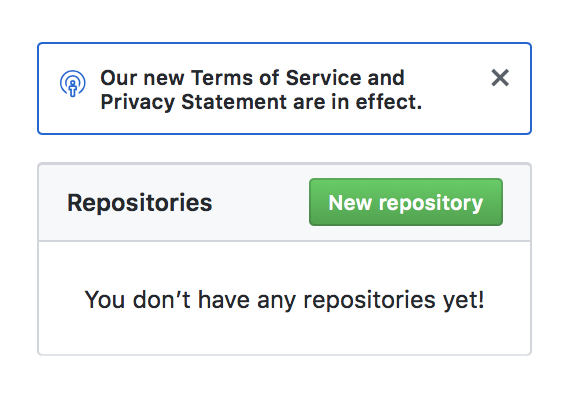
\includegraphics[width=.75\textwidth]{Figures/akunGit/6.PNG}}
\caption{Menampilkan Repository}
\label{6}
\end{figure} 
\item Selanjutnya pada gambar \ref{7} merupakan menu yang digunakan untuk mencatat segala bentuk aktivitas kita di dalam repository
\item Melalui menu ini juga kita dapat mencari repository yang dibuka secara public melalui tab \textbf{Discover Repositories}
\begin{figure}[!htbp]
\centerline{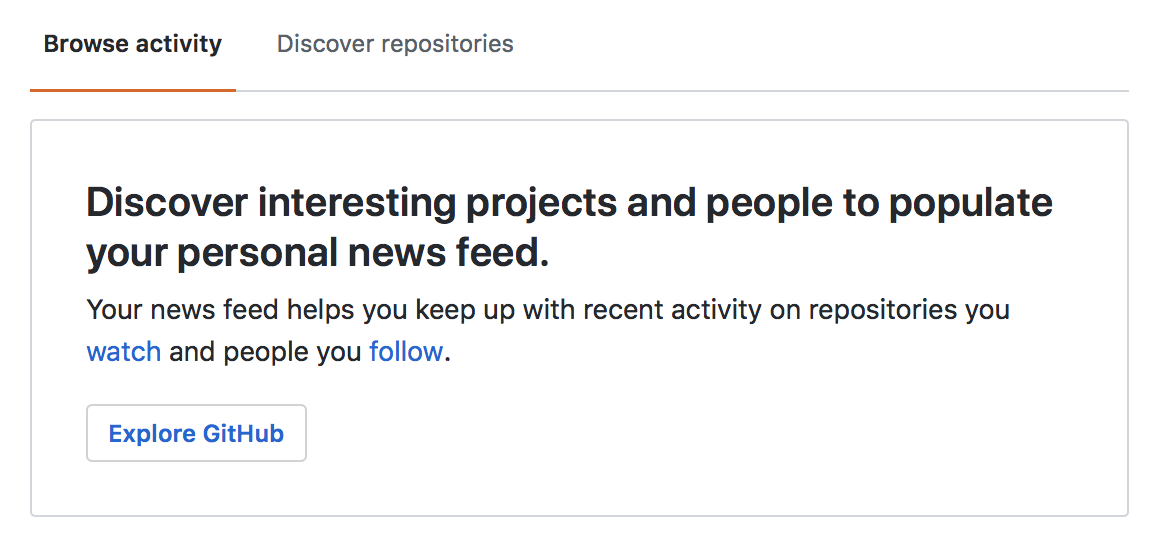
\includegraphics[width=.75\textwidth]{Figures/akunGit/7.PNG}}
\caption{Discover Repositories}
\label{7}
\end{figure} 
\item Selanjutnya untuk membuat project baru (repository) klik tombol start a project seperti pada gambar \ref{8}
\begin{figure}[!htbp]
\centerline{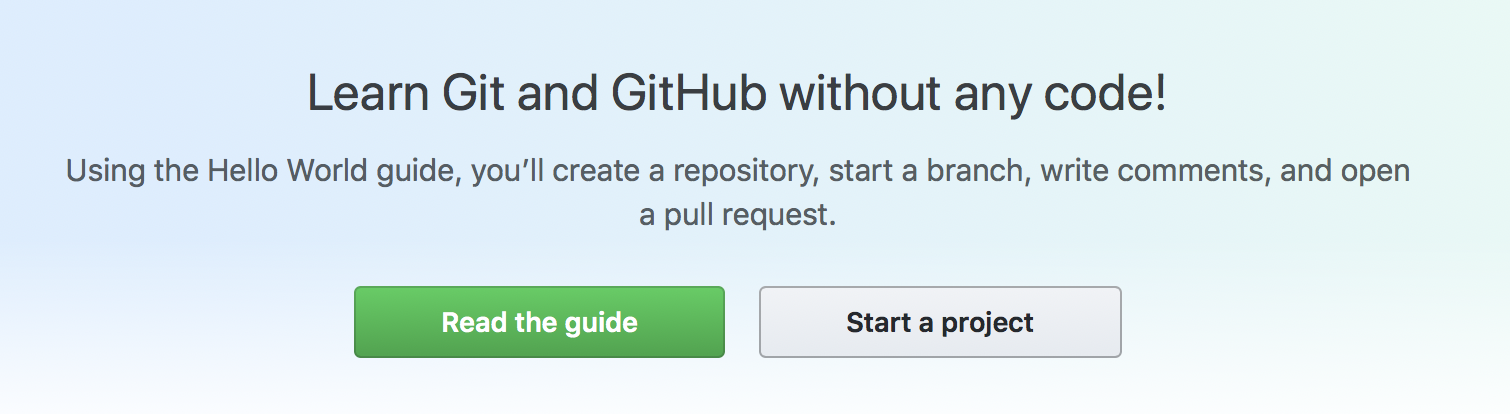
\includegraphics[width=.75\textwidth]{Figures/akunGit/8.PNG}}
\caption{Start a Project}
\label{8}
\end{figure} 
\end{enumerate}

\section{Membuat Akun Gitlab}
Gitlab ini sama halnya dengan Github dimana kalangan developer biasanya menggunakan Gitlab sebagai tempat penyimpanan project-project open source sehingga dapat dikembangkan oleh programmer lain baik sebagai team maupun individual. Namun, terdapat perbedaan antara Github dan Gitlab sebagai berikut :
\begin{itemize}
\item Menawarkan public project dan private project
\subitem fitur public dan private pada Gitlab dapat kita akses secara gratis, beda halnya dengan Github yang hanya menyediakan public saja yang secara gratis.
\item Snippet support 
\subitem pada Gitlab terdapat fitur ini yaitu memungkinkan pengguna dapat berbagi potongan kecil source code tanpa membagikan keseluruhan code.
\item Progress status
\subitem Pada Gitlab para developer dapat memberikan label dalam project yang sedang dikerjakan dengan label \textit{Work in Progress} sehingga dapat memberikan kejelasan atas project yang sedang dibuat atau dikembangkan.
	Setelah mengetahui sedikit tentang perbedaan antara Github dan Gitlab, kita akan mencoba membuat akun Gitlab. Sebelum kita membuat ternyata Gitlab terintegrasi dengan Github :
\end{itemize}

\begin{enumerate}
\item Pertama, buka browser dan masukkan alamat Gitlab dengan url : \textbf{https://gitlab.com} seperti pada gambar \ref{urlgitlab}
\begin{figure}[!htbp]
\centerline{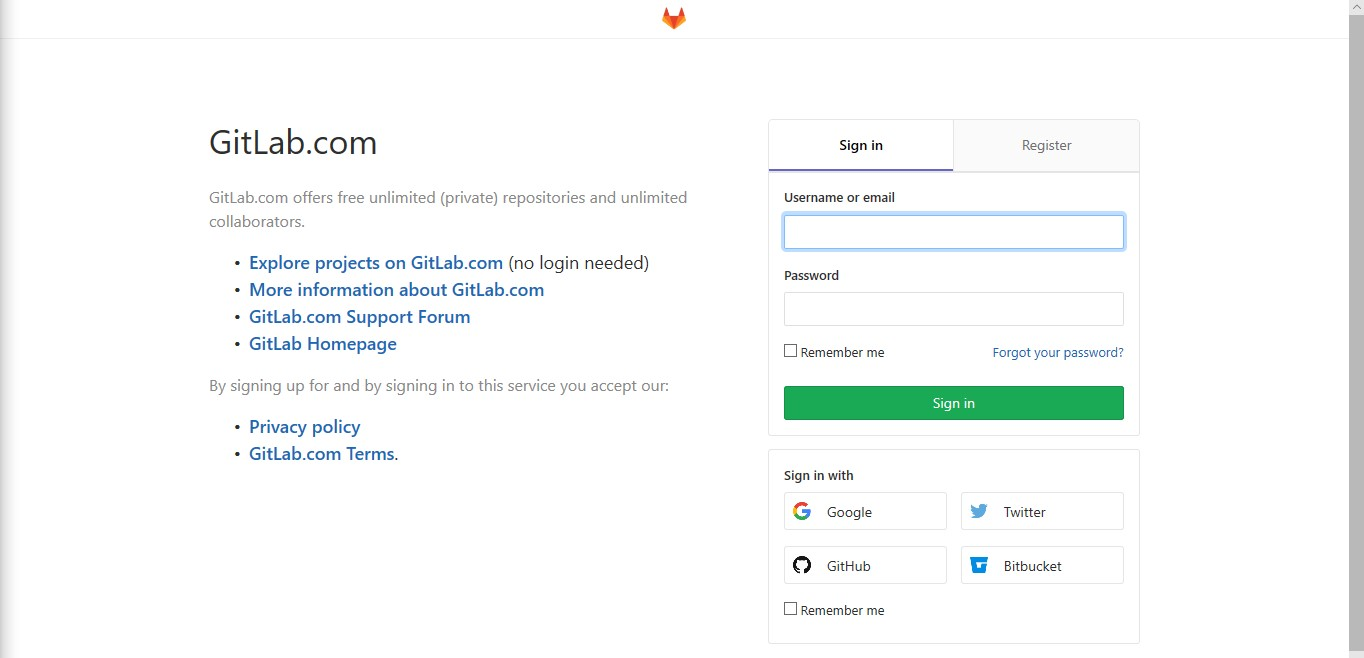
\includegraphics[width=.75\textwidth]{Figures/akunGit/gitlab1.jpg}}
\caption{URL Gitlab}
\label{urlgitlab}
\end{figure}

\item Karena Gitlab ini terintegrasi dengan Github, maka jika sudah mempunyai akun Github kita tinggal sign in menggunakan akun Github seperti pada gambar \ref{signingithub}
\begin{figure}[!htbp]
\centerline{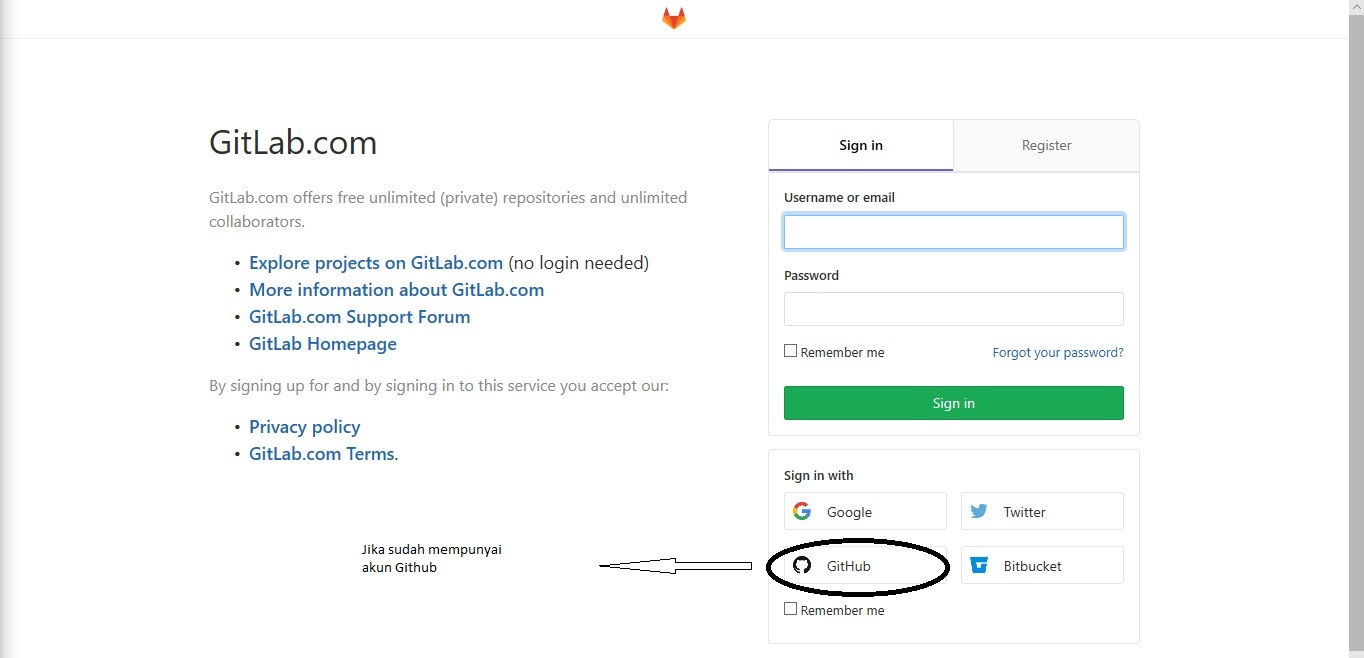
\includegraphics[width=.75\textwidth]{Figures/akunGit/gitlab2.jpg}}
\caption{Sign in with Github}
\label{signingithub}
\end{figure}

\item Setelah itu, kita authorized akun Github ke dalam akun Gitlab

\item Setelah berhasil maka kita diarahkan ke halaman seperti pada gambar \ref{hlmgitlab}
\begin{figure}[!htbp]
\centerline{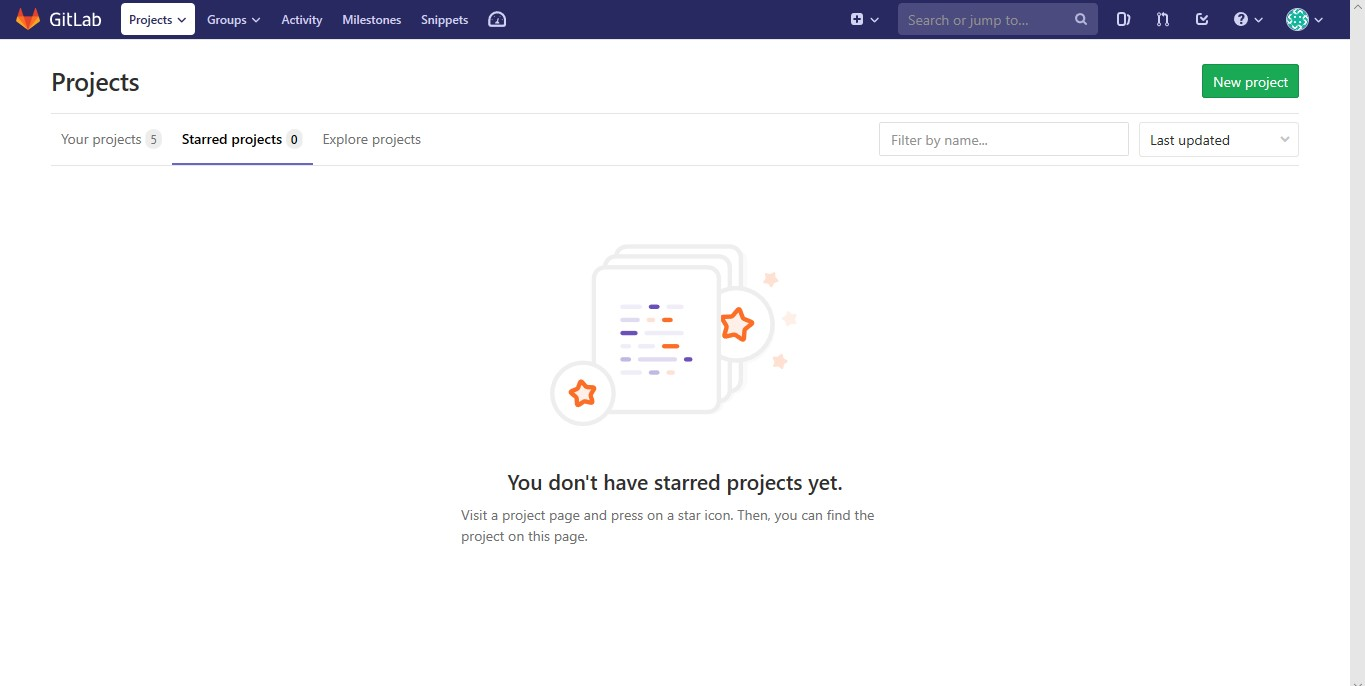
\includegraphics[width=.75\textwidth]{Figures/akunGit/gitlab3.jpg}}
\caption{Halaman Gitlab}
\label{hlmgitlab}
\end{figure}

\item Selanjutnya kita akan configurasi SSH key pada Gitlab \ref{sshkey}
\begin{figure}[!htbp]
\centerline{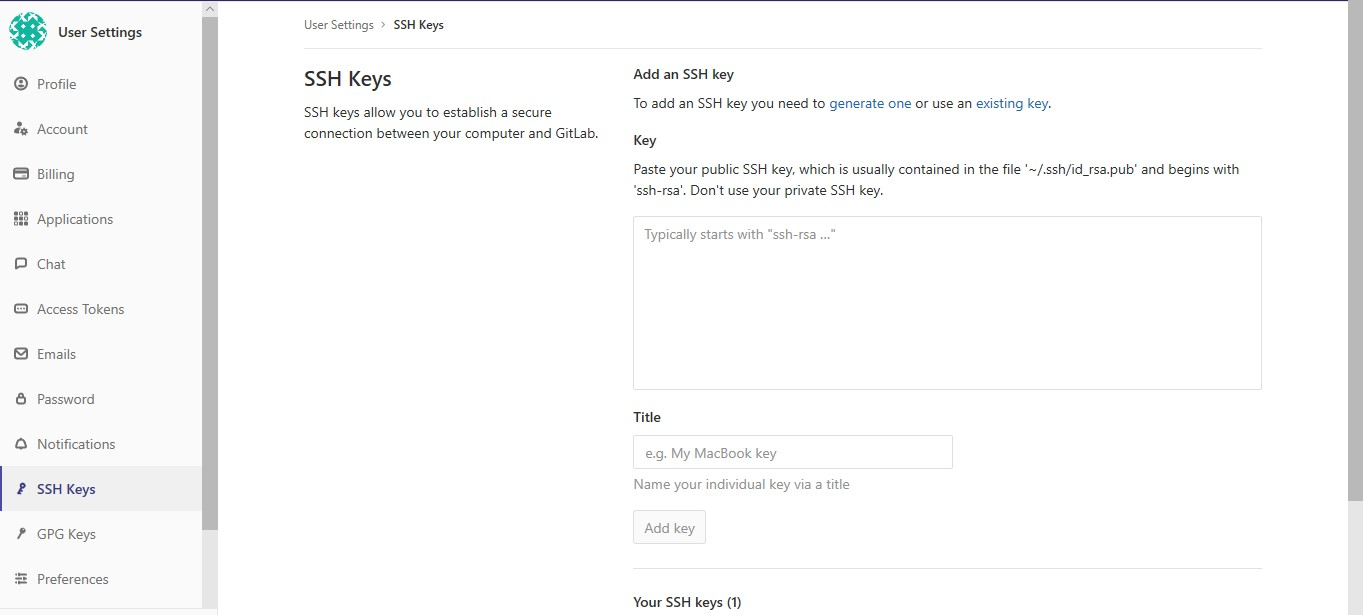
\includegraphics[width=.75\textwidth]{Figures/akunGit/gitlab5.jpg}}
\caption{SSH key}
\label{sshkey}
\end{figure}

\item kita ambil SSH key yang sudah kita buat pada akun Github, kita buka Git Bash ketikan seperti gamabar \ref{sshbash}
\subitem \textbf{cd .ssh}, kita masuk ke direktori .ssh
\subitem \textbf{ls}, untuk melihat list file yang terdapat pada direktori .ssh
\subitem \textbf{cat id\_rsa.pub}, lalu kita panggil ssh key dalam file id\_rsa.pub
\begin{figure}[!htbp]
\centerline{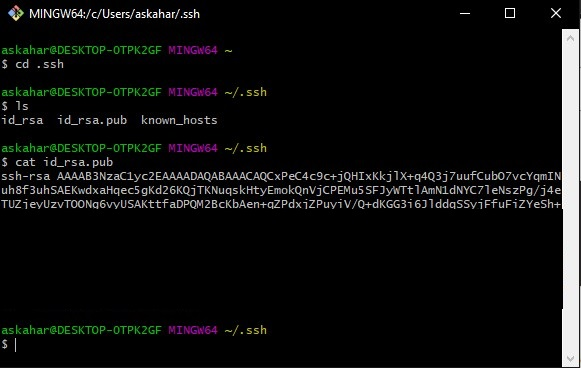
\includegraphics[width=.75\textwidth]{Figures/akunGit/gitlab6.jpg}}
\caption{Ambil SSH key menggunakan Git Bash}
\label{sshbash}
\end{figure}

\item Setelah kita mendapatkan SSH key kita, lalu kita copy paste ke dalam SSH key Gitlab spserti pada gambar \ref{copypaste}
\begin{figure}[!htbp]
\centerline{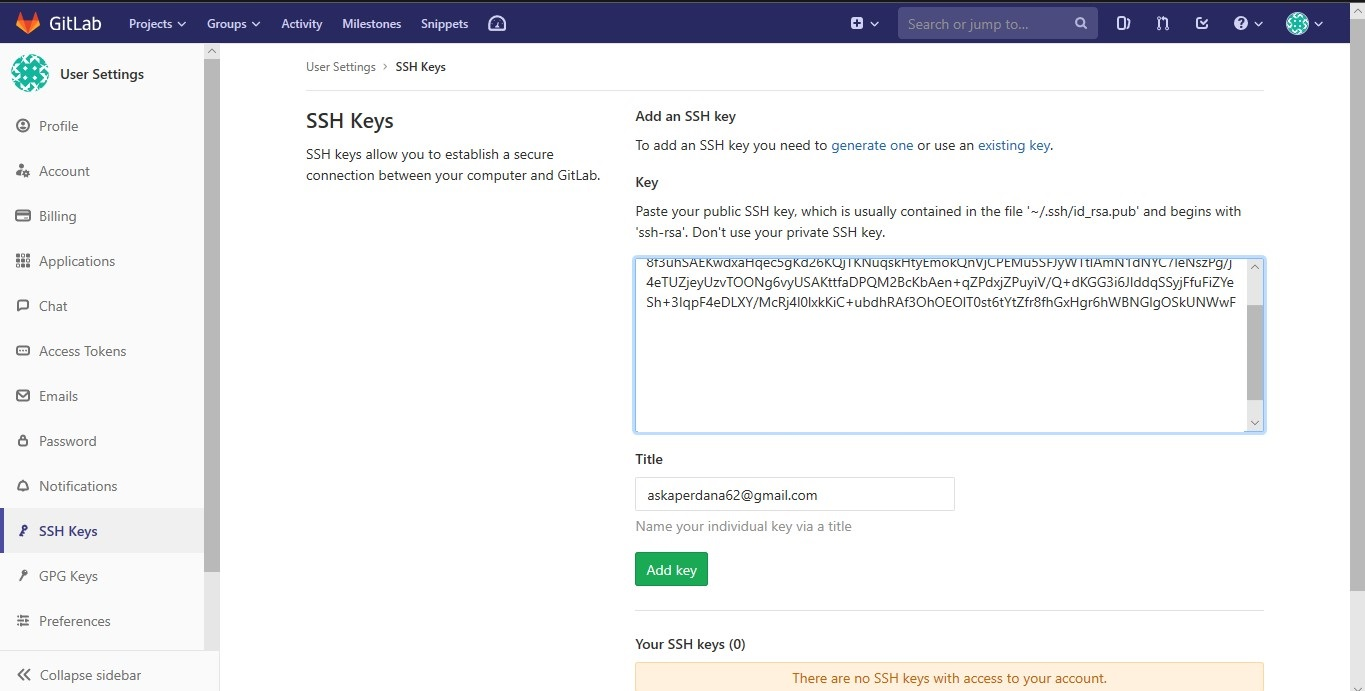
\includegraphics[width=.75\textwidth]{Figures/akunGit/gitlab7.jpg}}
\caption{Copy paste SSH key Bash ke dalam SSH key Gitlab}
\label{copypaste}
\end{figure}

\item Selanjutnya jika sudah memasukkan SSH key kita dapat memulai menggunakan Gitlab kita, untuk membuat project baru klik tombol new project seperti pada gambar \ref{newproject}
\begin{figure}[!htbp]
\centerline{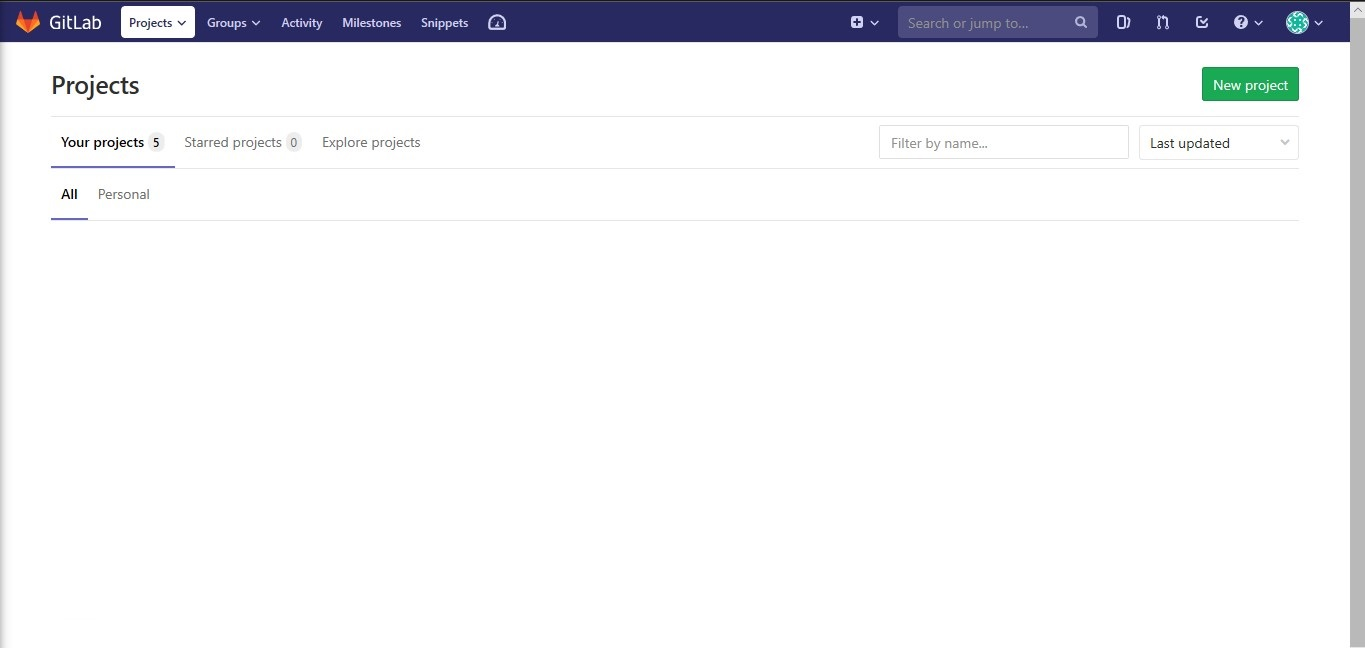
\includegraphics[width=.75\textwidth]{Figures/akunGit/gitlab8.jpg}}
\caption{Membuat Project baru}
\label{newproject}
\end{figure}
\end{enumerate}